Plusieurs expérimentations sont nécéssaires pour se convaincre du bon fonctionnement global de la vérification de la sûreté d'automates à files par apprentissage actif. Trois cas sont retenus.
\begin{itemize}
  \item L'algorithme s'arrête en déclarant l'automate sûr.
  \item L'algorithme s'arrête en déclarant l'automate comme étant à risque.
  \item L'algorithme ne s'arrête pas.
\end{itemize}

Le programme a été exécuté sur différents exemples $F$ et le résultat a été confirmé par rapport à l'automate étudie. L'évolution de l'ADF $A$ candidat pour accepter $AL(F)$ a été exportée sous forme d'images. Dans ces images, représentant des ADF, une notation a été établie.
\begin{itemize}
  \item Une transition sur $ti$ dans l'image représente une transition sur $\theta_i$ dans $A$.
  \item Une transition sur $bi$ dans l'image représente une transition sur $\bar{\theta}_i$ dans $A$.
  \item Une transition sur $si$ dans l'image représente une transition sur $t_{q_i}$ dans $A$.
\end{itemize}



\subsection{Exécution avec arrêt}

L'automate à files $F$ de la figure \ref{fig:fex2} permet d'étudier les deux premiers cas.

\begin{figure}[H]
    \centering
    \begin{tikzpicture}[->,>=stealth',shorten >=1pt,auto,node distance=5cm, semithick, bend angle=10]

    \tikzstyle{every state}=[circle]


    \node[initial, state]   (0)                         {$q_0$};
    \node[state]            (1) [above right of=0]      {$q_1$};
    \node[state]            (2) [below right of=0]      {$q_2$};

    \path
    (0) edge [bend left=10] node {$\theta_0(a!0)$} (1)
    (1) edge [bend left=10] node {$\theta_1(a?0)$} (0)
    (2) edge node {$\theta_2(a?1)$} (1)
    ;
    \end{tikzpicture}
    \caption{Automate à files $F$}\label{fig:fex2}
\end{figure}

La question de la sûreté de cet automate à files $F$ est posée pour deux ensembles $\mathcal{W}$:

\begin{itemize}
  \item $\mathcal{W}_1$ : Toute configuration de l'automate à files où l'état courant est $q_1$.
  \item $\mathcal{W}_2$ : Toute configuration de l'automate à files où l'état courant est $q_2$.
\end{itemize}

Voici les différentes itérations de l'algorithme avant l'arrêt du programme.

\begin{enumerate}

\item L'automate $A_1$ acceptant le langage $L=\{t_{q_0}\}$ est proposé (figure \ref{fig:fina1}). Celui-ci est refusé et un contre-exemple est fourni : $\gamma=\theta_0 t_{q_1}$. En effet, $A_1$ n'accepte pas $\gamma$ alors qu'il existe bien une exécution valide de $F$ pour ce mot.

\begin{figure}[H]
  \centering
  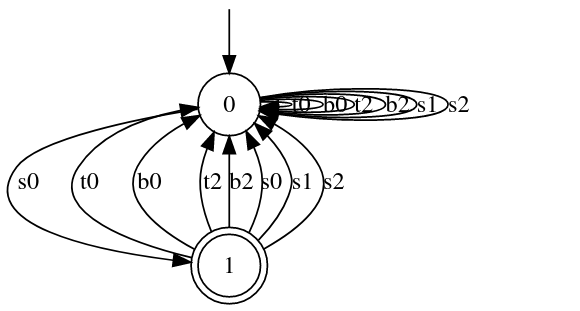
\includegraphics[width=0.4\linewidth]{res/minimalist_0}
  \caption{Automate $A_1$ lors du premier appel à l'oracle d'équivalence}\label{fig:fina1}
\end{figure}

\item L'automate $A_2$ de la figure \ref{fig:fina2} est proposé. Il est refusé et le contre-exemple $\gamma=\theta_1 t_{q_1}$ est retourné. En effet, il est accepté par $A_2$ mais ne peut pas être exécuté par $F$.
\begin{figure}[H]
  \centering
  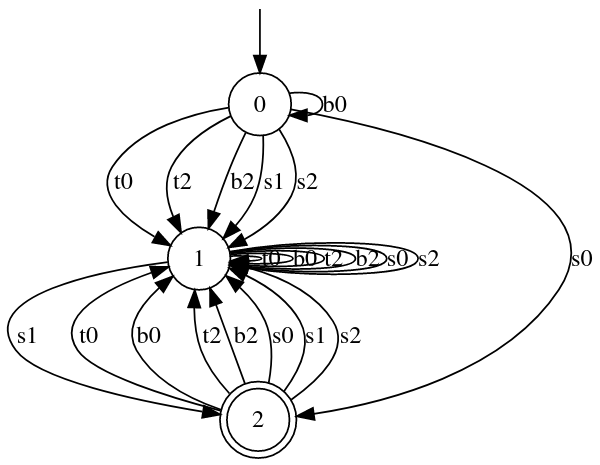
\includegraphics[width=0.4\linewidth]{res/minimalist_1}
  \caption{Automate $A_2$ lors du second appel à l'oracle d'équivalence}\label{fig:fina2}
\end{figure}

\item L'automate $A_3$ de la figure \ref{fig:fina3} est proposé. Aucun contre-exemple n'est trouvé contre $L(A)=AL(F)$. Alors, les ensembles $\mathcal{W}$ sont évalués.
\begin{figure}[H]
  \centering
  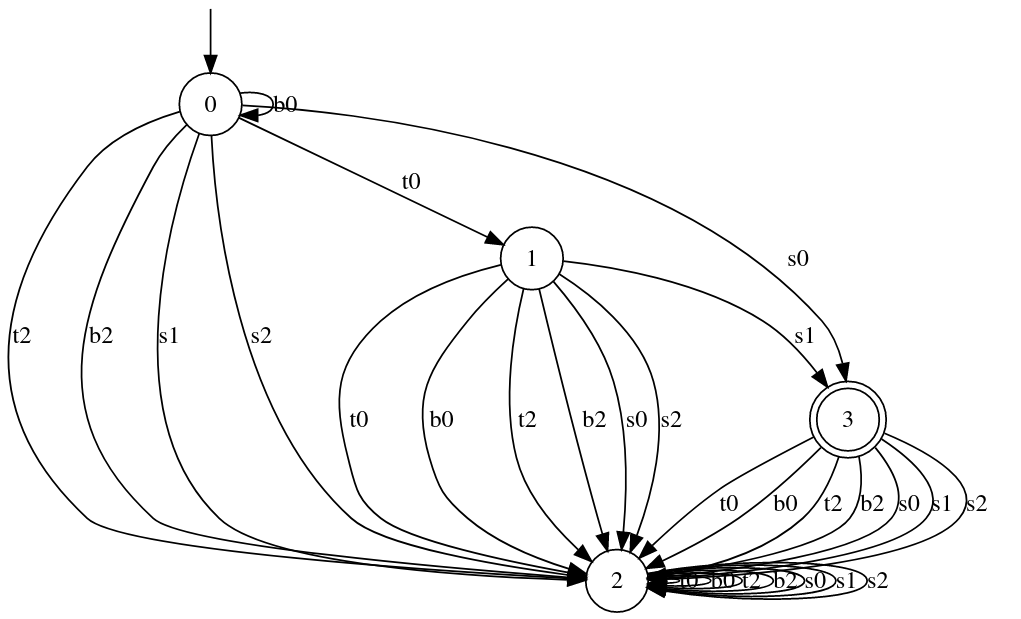
\includegraphics[width=0.6\linewidth]{res/minimalist_2}
  \caption{Automate $A_3$ lors du troisième appel à l'oracle d'équivalence}\label{fig:fina3}
\end{figure}

D'après $A_3$, il est possible de suivre le chemin $\gamma=\theta_1t_{q_1}$. Ce chemin passe par $q_1$. $F$ est alors déclaré comme à risque pour $\mathcal{W}_1$.

Par contre, aucun chemin valide ne passe par $q_2$. $F$ est alors déclaré comme sûr pour $\mathcal{W}_2$.
\end{enumerate}



\subsection{Exécution sans arrêt}

Pour cette troisième possibilité, l'algorithme qui ne s'arrête pas, l'automate à files $F$ utilisé est donné à la figure \ref{fig:fifo2}. Au nom des transitions près, indexées à partir de zéro, il s'agit du même automate à file que celui de la figure \ref{fig:fifo1}.

\begin{figure}[H]
  \centering
  \begin{tikzpicture}[->,>=stealth',shorten >=1pt,auto,node distance=2.5cm, semithick, bend angle=10]

    \tikzstyle{every state}=[circle]

    \node[initial,state] (A)                    {$q_0$};
    \node[state]         (B) [above right= 1cm and 3 cm of A] {$q_1$};
    \node[state]         (C) [below right= 1cm and 3 cm of A] {$q_2$};
    \node[state]         (D) [above right= 1cm and 3 cm of C] {$q_3$};

    \path
    (A) edge node {$\theta_0(a!0)$} (B)
    (A) edge node[below left] {$\theta_1(a!1)$} (C)
    (B) edge node {$\theta_3(a?0)$} (D)
    (B) edge[loop above] node {$\theta_2(b!1)$} (B)
    (C) edge node[below right] {$\theta_5(a?1)$} (D)
    (C) edge [loop below] node{$\theta_4(b!0)$} (C)
    (D) edge node[above] {$\theta_6(b?0)$} (A)
    ;
  \end{tikzpicture}
  \caption{Automate à files $F$}\label{fig:fifo2}
\end{figure}

Voici le suivi de l'exécution du programme jusqu'à ce qu'un motif récurrent émerge, suggérant que l'exécution ne s'arrête pas.

\begin{enumerate}
  \item L'automate $A_1$ acceptant le langage $L=\{t_{q_0}\}$ est proposé (figure \ref{fig:fina1}). Celui-ci est refusé et un contre-exemple est fourni : $\gamma=\theta_0 t_{q_1}$. En effet, $A_1$ n'accepte pas $\gamma$ alors qu'il existe bien une exécution valide de $F$ pour ce mot. C'est la même situation que dans la sous-section précédente.
  \begin{figure}[H]
    \centering
    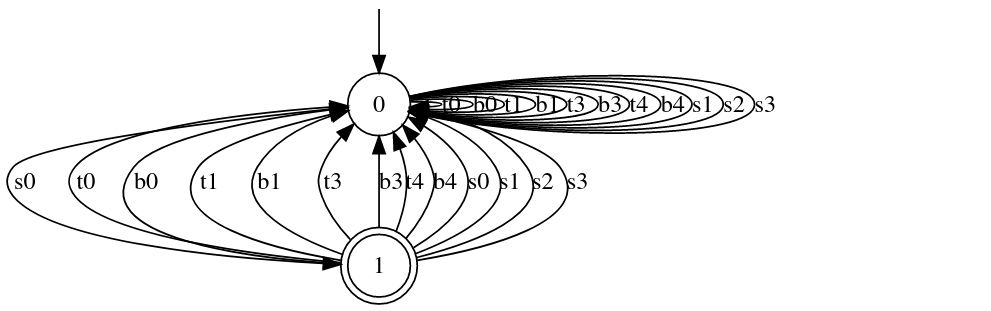
\includegraphics[width=0.6\linewidth]{res/andre_0}
    \caption{Automate $A_1$ lors du première appel à l'oracle d'équivalence}\label{fig:andre0}
  \end{figure}
  \item L'automate $A_2$ est proposé et refusé. Le contre-exemple $\gamma=\bt_0 t_{q_3}$ est retourné. En effet, le chemin $w=\theta_0.\theta_3$ est valide dans $F$, mène bien à $q_3$ et $\mathcal{A}(w)=\gamma$. $\gamma$ aurait dû être accepté par $A_2$.
  \item L'automate $A_3$ est proposé et refusé. Le contre-exemple $\gamma=\theta_3 t_{q_3}$ est retourné. $\gamma$ ne correspond à aucune exécution valide de $F$, ce mot ne devrait pas accepter par $A_3$.
  \item L'automate $A_4$ est proposé et refusé. Le contre-exemple $\gamma=\bt_1\theta_3 t_{q_3}$ est retourné, étant accepté par $A_4$ à tort.
  \item L'automate $A_5$ est proposé et refusé. Le contre-exemple $\gamma=\bt_1\bt_4\theta_4 t_{q_0}$ est retourné, le mot $\gamma$ n'étant pas accepté par $A_5$ alors qu'il devrait l'être.
  \item L'automate $A_6$ de la figure \ref{fig:andre6} est proposé. Il a été simplifié depuis l'automate original par souci de lisibilité.
  \begin{figure}[H]
    \centering
    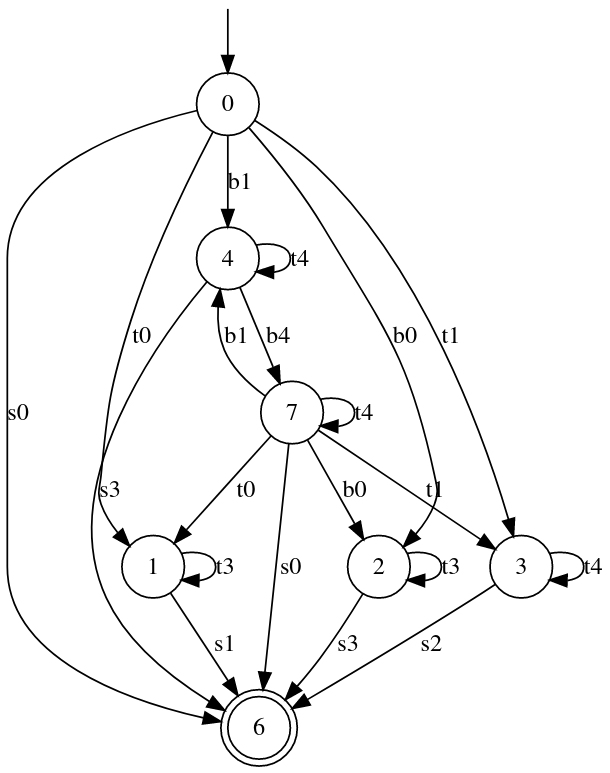
\includegraphics[width=0.4\linewidth]{res/andre_6}
    \caption{Automate $A_6$ lors du sixième appel à l'oracle d'équivalence}\label{fig:andre6}
  \end{figure}
  On peut déjà y remarquer une transition sur $\bt_4$ entre les états 4 et 7. Cependant, ce n'est pas suffisant. Un contre-exemple $\gamma=\bt_1\bt_4\bt_4\bt_0t_{q_0}$ est fourni. Le mot $\gamma$ n'est pas accepté par $A_6$ alors qu'il devrait l'être. Auquel cas, une exécution valide dans $F$ est : $w=\theta_1\theta_4\theta_4\theta_5\theta_6\theta_0\theta_3\theta_6$. $w$ est bien une exécution valide dans $F$ menant à $q_0$. De plus, $\mathcal{A}(w)=\gamma$.
  \item L'automate $A_7$ de la figure \ref{fig:andre7} est proposé. Il est également simplifié pour plus de lisibilité.
  Néanmoins, il reste plus complexe que $A_6$. En particulier, on peut noter l'apparition des états $8$ et $9$, servant à compter une utilisation de $\theta_4$ supplémentaire.
  Un contre-exemple $\gamma=\bt_1\bt_4\bt_4\bt_4\bt_0\bt_0t_{q_0}$ est fourni. Il est semblable au contre-exemple précédent. En réalité, il contient une utilisation de $\theta_4$ en plus.

  \begin{figure}[H]
    \centering
    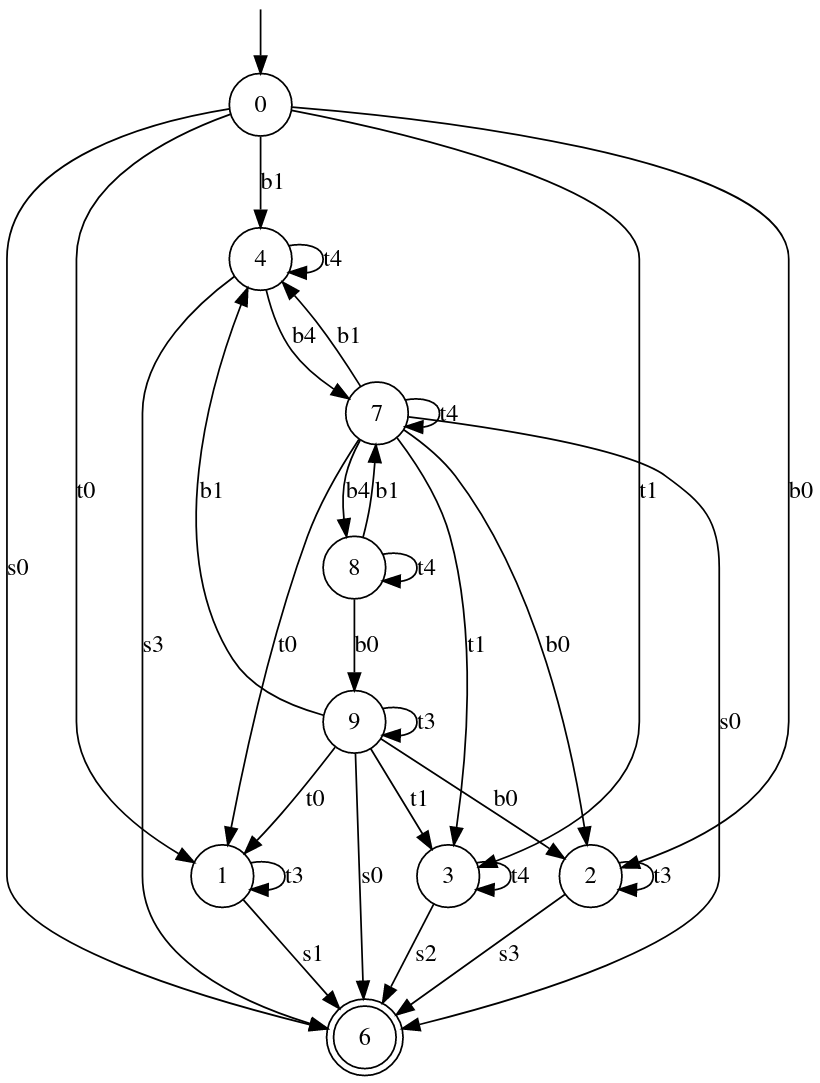
\includegraphics[width=0.6\linewidth]{res/andre_7}
    \caption{Automate $A_7$ lors du septième appel à l'oracle d'équivalence}\label{fig:andre7}
  \end{figure}

\end{enumerate}

À partir de là, l'automate se complexifie d'itération en itération, cherchant en vain à trouver un langage régulier permettant de garder le compte du nombre de transitions $\theta_4$ suivies. C'est un comportement cohérent au vu de l'automate $F$. Cet automate simple fait partie de la classe des automates à files pour lesquels la méthode LeVer est insuffisante.
